\chapter[Draft of the application]{Draft of the application}
To handle all these problems that have been described above within the section about the current situation, we will create a smartphone application that gets supported by a backend web-server. The master thesis will handle the planning respectively cost estimation of the different parts/features of the system and will, after the needed technologies/frameworks are elaborated and evaluated, include a prototypical implementation of the needed components.
But at first, we will start with the first step in a development process; the requirements engineering.

\section{Requirements engineering}
Because the HiP-Application will be developed closely together with our \textit{costumer}, other working-groups at the university of paderborn, the whole process starts with the requirements engineering phase.

First of all, a requirement is defined as "[...]A condition or capability that must be met or possessed by a system or system component to satisfy a contract, standard, specification, or other formally imposed documents[...]" (\cite{IEEEReq}).

We started the development with a requirements engineering meeting together with our \textit{customer} and ended up with a couple of cards with written user stories. Afterwards, these stories got refined to concrete requirements, which are measurable and prioritized. A complete list of all requirements, which were derived from these user stories, can be found within the appendix in Table \ref{RequirementsFrontend} and \ref{RequirementsBackend}. These requirements can directly be used to derive test cases from them, which is good because we will use a \ac{TDD} driven development approach in every sprint. 

In the following, we will explain the two parts of the application separately.

\section{Backend (Web-Server)}
Another important part of the system is contained within the backend-web-server. The backend should contain the whole data handling and assessment. The students should be able to add data to the system (e.g., a textual article, graphics, \ac{AR}-data, etc.) and to modify existing data via a \ac{CMS}. These entries get reviewed, for example by the course supervisor, and unlocked for the frontend application. To do this, the backend needs features like annotations and highlighting, which should be private for a specific user. By using this, the supervisor can evaluate the given texts right within the \ac{CMS} and give his final judgement. If the supervisor is not satisfied with the quality of the given text, he should be able to send the document back to the student, to get a revised and updated version of the document. If the supervisor is satisfied, he can unlock the information for showing in the frontend application.

The data should be stored in a way that it can be shown within an \ac{AR}-environment in the smartphone application. Of course, we will need some mechanism to structure the data, for example tags or stored categories. This kind of information (especially tags) are also very important for the described filtering techniques on the client side.

\begin{figure}[th]
\centerline{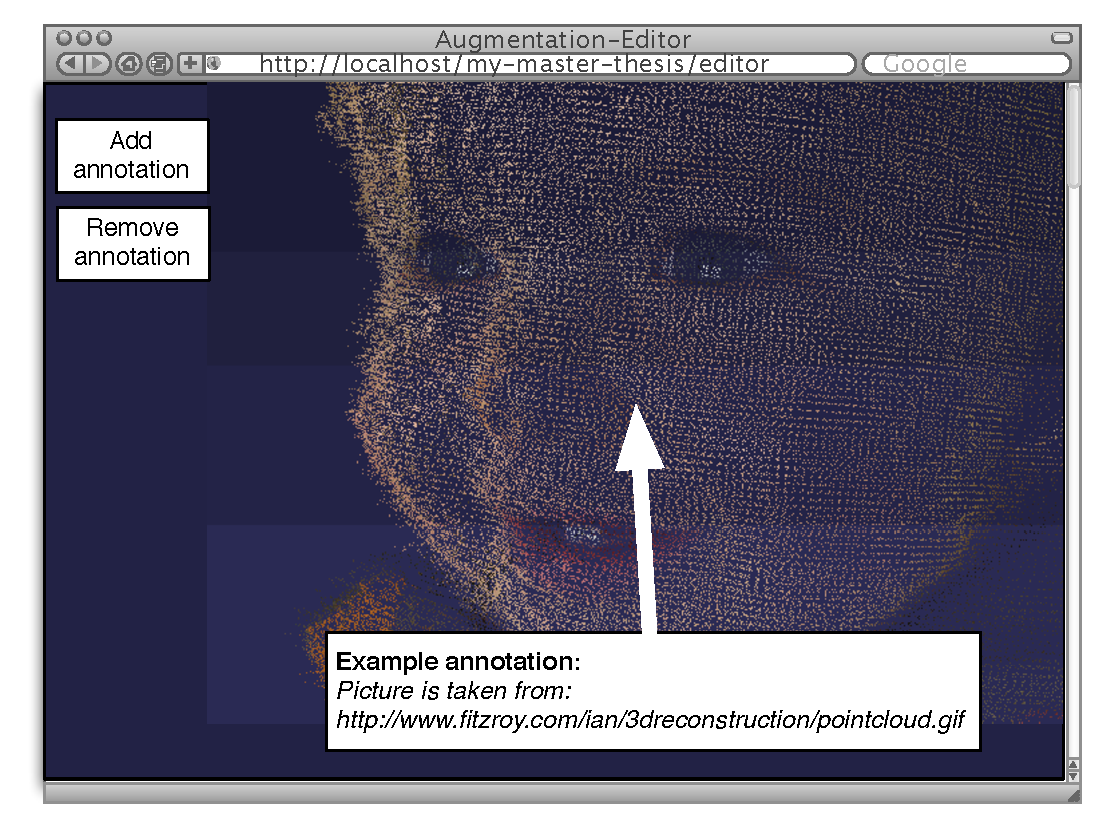
\includegraphics[width=1\textwidth]{gfx/mockup_web_1}}
\caption{A mockup showing the augmentation editor that will be included in the web-application. The editor will be used to edit the point-clouds, which have been added with the help of the smartphone-application}
\label{web1}
\end{figure}

Furthermore, the backend should include a way to modify the point-clouds of the objects that has been scanned with the smartphone application. It will need features to add annotations directly to these point-clouds to show them afterwards within the \ac{AR}-environment. This editor will be created on the basis of \ac{HTML5} and \ac{WebGL}. A mockup of this site is shown in Figure \ref{web1}. These annotations should also be assessable and (un-)lockable for the supervisor. 

\subsection{Cost estimation of the backend}

\subsection{Input data/content via CMS in the system}

\subsection{Manage content as a reviewer}

\subsection{Including a 3D-Tooling system for point-clouds (WebGL)}

\section{Frontend (App)}
\begin{figure}[th]
\centerline{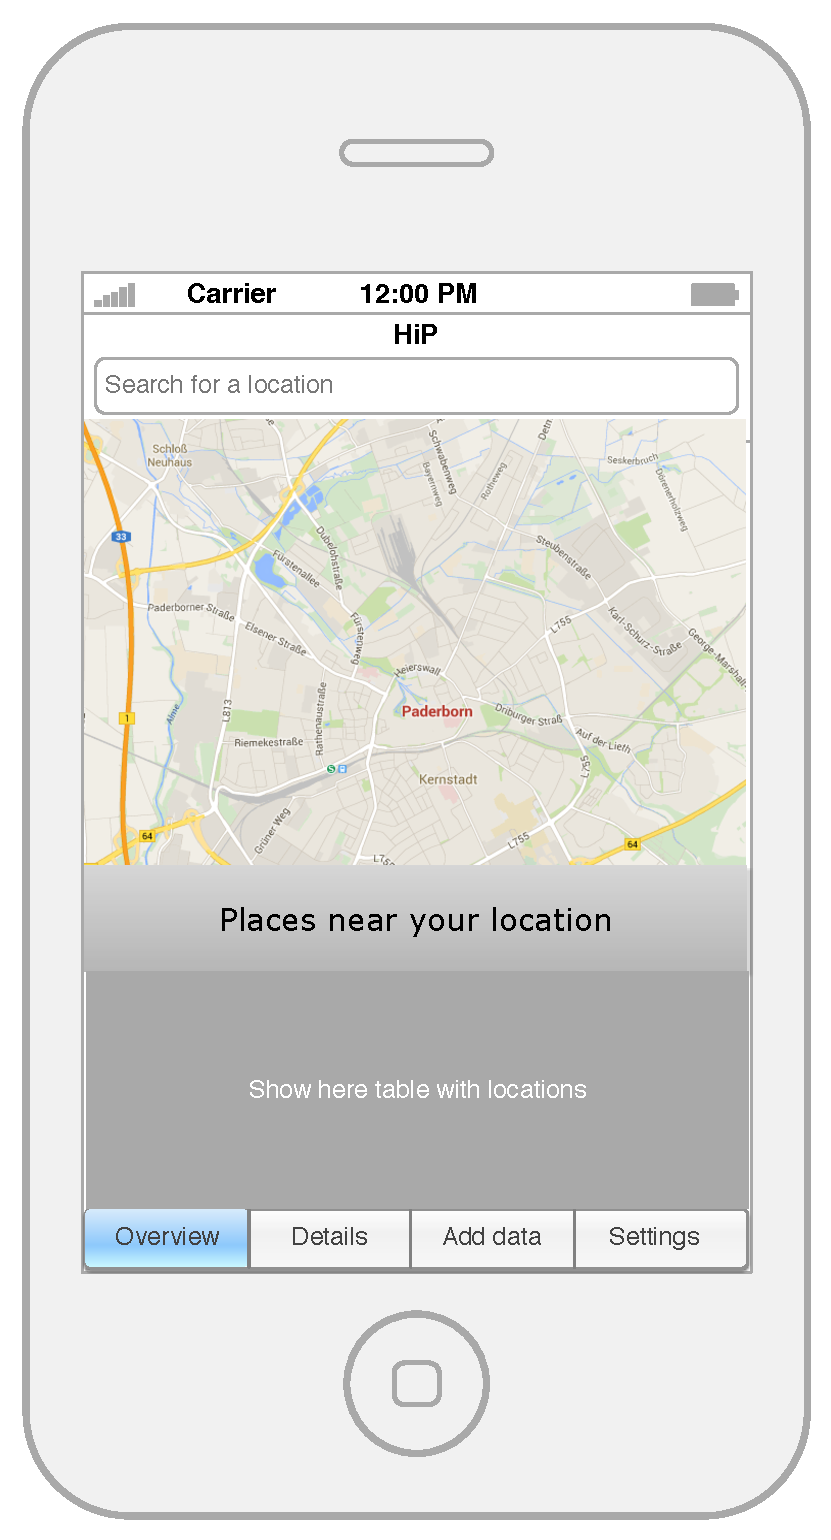
\includegraphics[width=0.5\textwidth]{gfx/mockup_app_1}}
\caption{A mockup showing the main page of the frontend application showing a map of paderborn and a general overview about the UI-elements}
\label{app1}
\end{figure}

The smartphone application is the part of the system that gets shipped to the end-user (respectively downloaded via an App-Store like Google-Play). The user can use the app to find interesting places respectively objects in Paderborn and is able to start a navigation to the place/object easily. Furthermore, the user can get an overview about all places in Paderborn by activating a map that shows all entries within the system. A mockup of this view is shown in Figure \ref{app1}. Of course, the user will be able to set up specific filters like 'show only art', 'show only historic buildings' or 'use simplified language' to adapt the system to his own experiences and educational qualifications. Moreover, if the university courses would add information over years, the system will need filtering features like this to handle the complexity of the data.

After an user has reached an interesting place, he can use the details tab to switch into the \ac{AR}-mode. With this view, the user can use the smartphone-camera to embed information, which has been added via the backend, right into the picture of the object. An mockup of this view is shown in Figure \ref{app2}. 
To create a feasible input for the \ac{AR} system, the user should be able to scan objects in 3D right with his smartphone application and send the data (i.e., a point-cloud of the scanned object), back to the web-server.  Afterwards, the user can add annotations to the point-cloud via the web-backend of the system.  

\begin{figure}[th]
\centerline{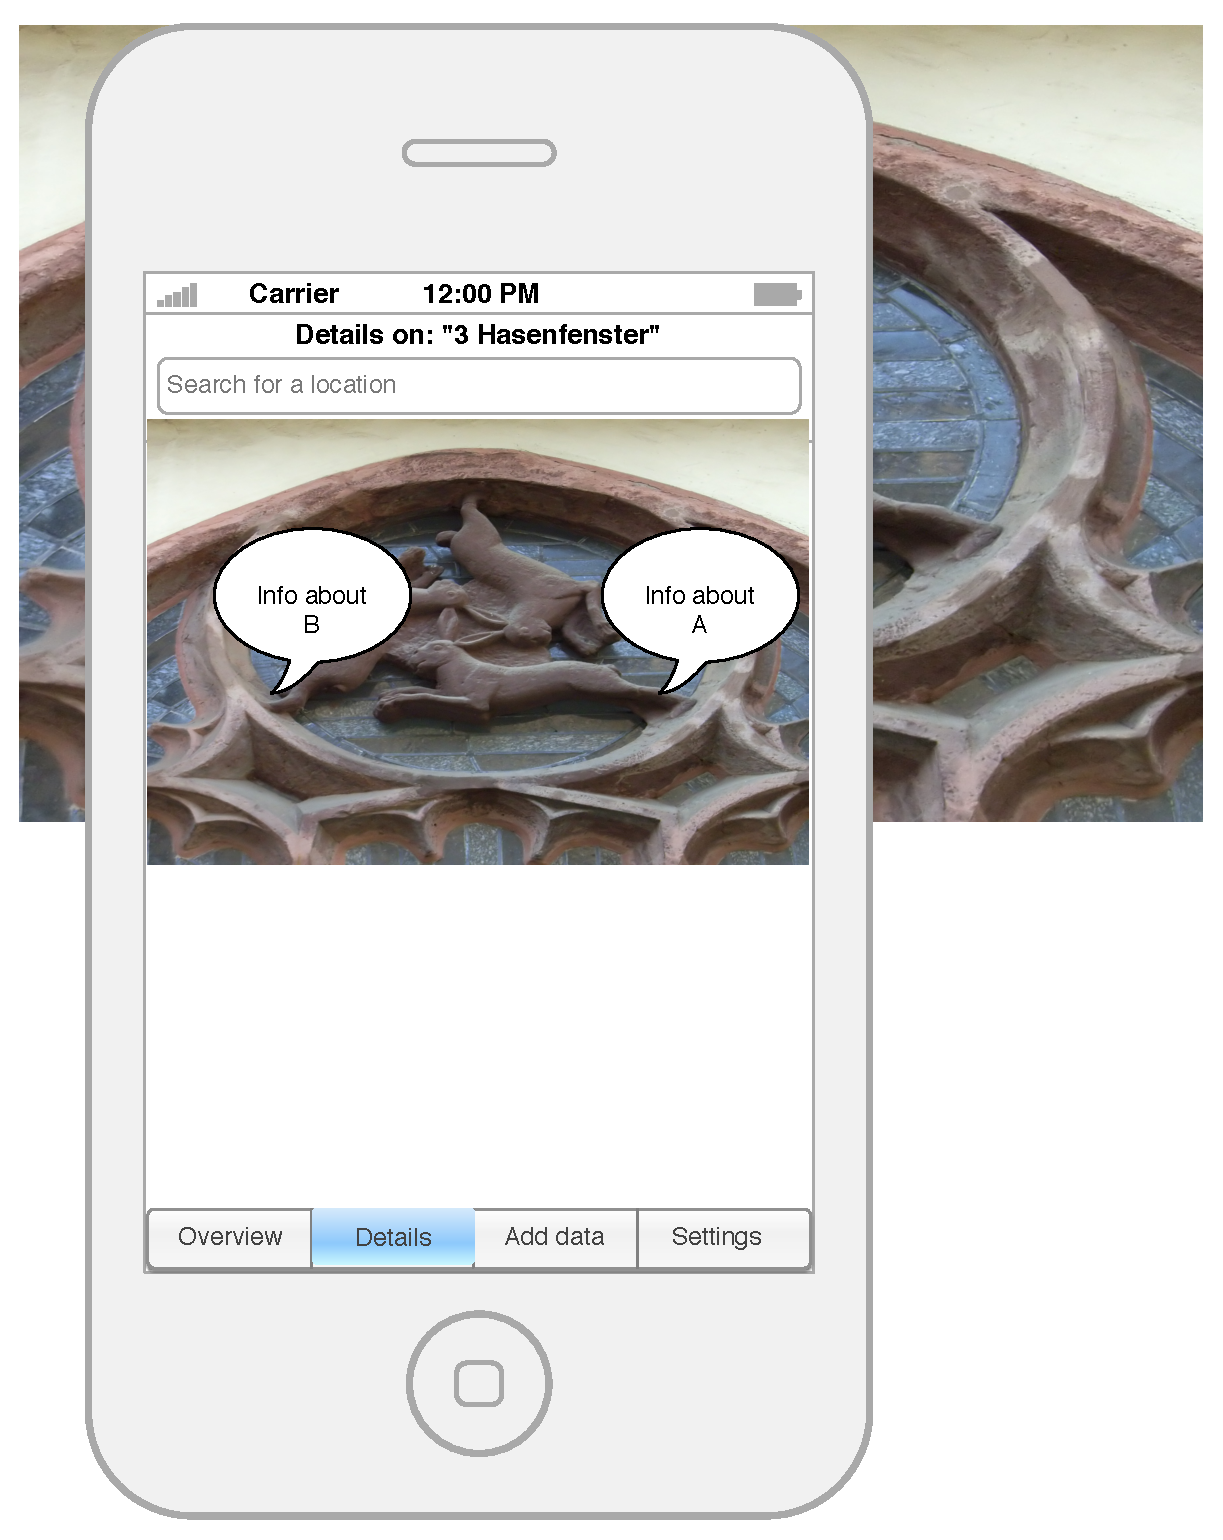
\includegraphics[width=0.7\textwidth]{gfx/mockup_app_2}}
\caption{A mockup showing the details page of the "Dreihasenfenster" while the camera of the smartphone is pointing to the window itself}
\label{app2}
\end{figure}

\subsection{Cost estimation of the frontend}				
  
\subsection{Input data into the system (scan objects and annotate them)} 

\subsection{Show close "interesting places" within a map /  via a overlay} 

\subsection{Navigation to "interesting places"}
				
\section{Interface}							 

\subsection{Data format for \ac{AR} files}